\section{DISEÑO DE INVESTIGACIÓN}
%http://recipp.ipp.pt/bitstream/10400.22/136/3/KDD-CRISP-SEMMA.pdf
%http://www.oldemarrodriguez.com/yahoo_site_admin/assets/docs/Documento_CRISP-DM.2385037

Uno de los pilares básicos en el diseño de una investigación es indicar el camino que se va a seguir en esta. Es importante establecer que estándar o norma se va a seguir en el desarrollo de un proyecto o una investigación. En esta investigación se va a utilizar la norma UNE 166006:2018 Gestión de la I+D+I: Sistemas de vigilancia e inteligencia. Esta norma está alineada con la norma UNE-EN ISO 9001 Sistema de Gestión de Calidad. 

La norma \citeA{une2018} tiene como objeto facilitar la formación y estructuración del proceso de recogida, análisis y comunicación de la información sobre el entorno de una organización. No solo muestra un proceso, sino que también establece roles, responsabilidades y políticas.

La \citeA{une2018} establece un proceso genérico para satisfacer los objetivos deseados y contemplar la realización de la vigilancia e inteligencia. Este proceso se divide en distintas etapas básicas. En la figura \ref{fig:UNEsquema} se puede observar cada etapa.

\begin{figure*}[h]
\centering
\caption{Proceso de la vigilancia e inteligencia. Recuperado de \protect\citeA{une2018}.}
 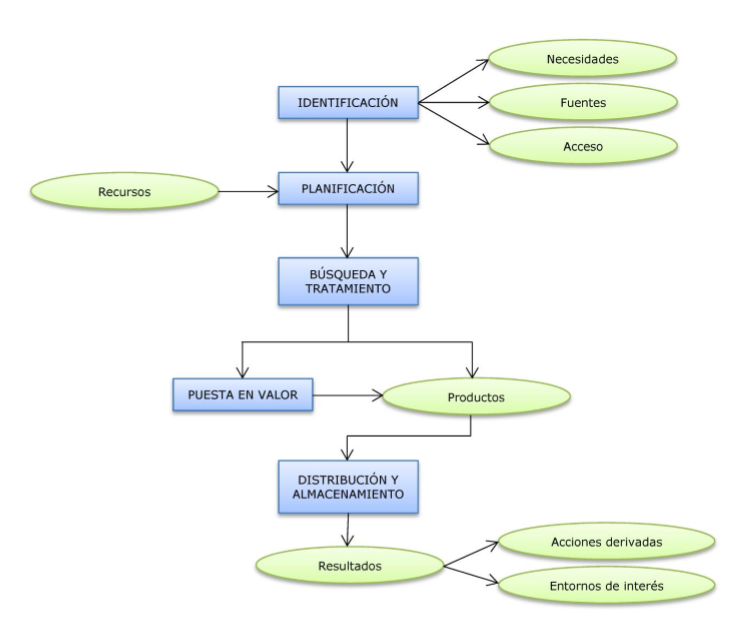
\includegraphics[width=0.8\textwidth]{recursos/UNEEsquema}
\label{fig:UNEsquema}
\end{figure*}


En los próximos puntos se va a describir las actividades que se van a realizar en este proceso.

\subsection{Identificación de necesidades, fuentes de información y medios de acceso}
\subsubsection{Identificación de necesidades de información}
Para realizar la identificación de las necesidades de información se va a partir de varios factores como son:
\begin{itemize}
\item las demandas esperadas o manifestadas por (en este caso) una unidad de la consejería de educación.
\item el análisis, la evolución de productos, procesos, materiales y tecnologías en el ámbito de la minería de datos educativos.
\end{itemize}

\subsubsection{Identificación de fuentes internas y externas de información}
Teniendo en cuenta las principales necesidades de información, se debe identificar las fuentes de información y recursos disponibles ya sean internos o externos a la organización. En este caso, se van a utilizar las siguientes fuentes:
\begin{itemize}
\item Fundamentalmente se va a utilizar documentos y recursos internos de la organización como van a ser: Repositorios documentales, carpetas locales, bases de datos, etc.

\item Personas con conocimientos o experiencias relacionadas con la necesidad de información. En este aspecto se van a realizar distintas reuniones con las personas encargadas de esta unidad de la consejería de educación. Para ello se realizaran reuniones con estos responsables. A partir de estas reuniones se obtendrán las fuentes de información.
\item Fuentes documentales a las que tiene acceso a la organización, ya sea en soporte físico (revistas, catálogos, etc.) como en soporte electrónico. Además, se utilizarán recursos de información en Internet (portales, noticias, redes sociales, foros, etc.). 
\item Documentación técnica como reglamentaciones, especificaciones, propiedad industrial e intelectual o normas.
\item Resultados de análisis existentes sobre las tendencias de futuro preferentemente en el ámbito educativo.
\end{itemize}

\subsection{Planificación de la realización de la vigilancia e inteligencia}
Para realizar la planificación del proceso, la \citeA{une2018} indica que se debe realizar una búsqueda de nuevas áreas desconocidas y realizar un seguimiento sistemático de novedades en áreas previamente identificadas.

Esta etapa del proceso se ha contemplado mediante una justificación teórica, donde se ha hecho una investigación acerca de las metodologías, técnicas y herramientas.

\subsection{Búsqueda y tratamiento de la información}

La información fundamentalmente se encuentra en bases de datos internas, no obstante, se va a acceder a bases de datos externas en caso de necesidad para cumplimentar la información. 

En este aspecto, se debe recurrir a la ayuda de personas con conocimientos sobre el estado de las bases de datos. Como cualquier organización, la consejería de educación maneja grandes volúmenes de datos, por tanto, se debe tener conocimiento sobre donde se puede encontrar la información que satisfaga con las necesidades. 

El desconocimiento del estado de las bases de datos conlleva la inversión de una gran cantidad de tiempo en la búsqueda de los datos relevantes. 

Una vez que se tienen los datos, muchas veces es necesario realizar un tratamiento de estos, que consiste en una limpieza y una normalización de los mismos. Muchas veces este tratamiento conlleva la conversión de datos, como por ejemplo fechas, corrección de datos, etc.

\subsubsection{Proceso de Extracción, Extracción y Carga}

Para realizar este tratamiento de datos se utilizará la técnica conocida como ETL (extracción, transformación y carga) que consiste básicamente en obtener los datos de la fuente de origen (bases de datos, ficheros Excel, ficheros JSON, etc.), seleccionar aquellos datos que convengan al estudio, transformarlos según las necesidades que se tenga y depurarlos (evitando así datos erróneos). \cite{prakash2017etl} \cite{matos2006metodologia},\cite{gour2010improve}.
Para realizar este tratamiento, se ha va a utilizar Pentaho BI, que es un conjunto de programas libres para realizar entre otras muchas actividades, las técnicas de ETL. Concretamente, se ha utilizado la herramienta Spoon para desarrollar esta técnica. 
Una vez que se tienen los datos limpios y estructurados, se pueden realizar dos operaciones:

\begin{enumerate}
\item  En primer lugar, se pueden almacenar dichos datos en una base de datos y seguir utilizando Pentaho BI para poder crear cuadros de mandos e informes. 
\item  En segundo lugar, se puede almacenar la información en un texto plano para poder trabajar con herramientas de análisis descriptivo y predictivo. Estos análisis se van a realizar a través del entorno y lenguaje de programación R, que es una referencia en el ámbito de la estadística.
\end{enumerate}


\subsubsection{Análisis Exploratorio}

%El análisis predictivo (también conocido como estadísticas predictivas) se encarga de resumir los datos en bruto para que puedan ser interpretados. Estos análisis son útiles ya que permiten aprender sobre comportamientos o patrones pasados e entender cómo pueden influir en los resultados futuros. En este tipo de análisis se van a utilizar tanto métodos gráficos como medidas resumen.

En primer lugar, se debe estudiar el tipo de datos de cada variable a investigar, se debe clasificar las variables según sean categóricas (dicotómicas o polinómicas) o numéricas (discretos o continuos). El tipo de datos permite decidir qué tipo de análisis estadístico utilizar.
Una vez que se tienen claro el tipo de datos utilizados, se van a utilizar los principales estadísticos como la media, la mediana, las desviaciones típicas, etc.
Posteriormente se va a utilizar la matriz de varianzas y covarianzas, que indicaran la variabilidad de los datos y la información sobre las posibles relaciones lineales entre las variables. 

Por otro lado, se va a estudiar la correlación de las variables mediante la matriz de correlación. Esta matriz contendrá los coeficientes de correlación.\cite{JMMarin}. La matriz de correlación, se utilizará fundamentalmente por pares entre las variables y la variable a predecir.

También se va a estudiar la matriz de correlaciones parciales, que estudia la correlación entre pares de variables eliminando el efecto de las restantes.\cite{JMMarin}

Los datos categóricos se van a representar en tablas de frecuencias, gráficos de barras y gráficos de sectores. Los datos numéricos se van a representar mediante histogramas, boxplot y diagramas QQ-Plot o Grafico Cuantil-Cuantil. \cite{Orellana2001}

Mediante el boxplot se puede observar aspectos como la posición, dispersión, asimetría, longitud de colas y los datos anómalos (outliers). 
El QQ-plot se va a utilizar para evaluar la cercanía de los datos a una distribución. \cite{Orellana2001}

%(https://www.sergas.es/gal/documentacionTecnica/docs/SaudePublica/Apli/Epidat4/Ayuda/Ayuda_Epidat_4_Analisis_descriptivo_Octubre2014.pdf)
Por otro lado, se va a complementar el análisis descriptivo mediante el aprendizaje no supervisado, donde también se extraerán otras características de los datos.

%En este apartado, se va a presentar la forma en la que se va a realizar la investigación. En primer lugar, se va a realizar un proceso ETL, posteriormente se va a realizar un análisis descriptivo mediante sus técnicas que se explicaran posteriormente, además se va a incluir técnicas de aprendizaje no supervisada en este análisis.
%Una vez que se ha realizado el análisis descriptivo, se va a realizar un análisis predictivo. En este análisis se va a utilizar técnicas de aprendizaje supervisadas.



\subsubsection{Aprendizaje automático}
\textbf{Aprendizaje No Supervisado}
\begin{enumerate}
\item Algoritmos de Clustering. El objetivo de estos algoritmos consiste en investigar si los datos pueden ser organizados en grupos o \textit{clusters} que posean características similares. %http://www.iesta.edu.uy/wp-content/uploads/2014/05/Escueladeverano_RegionalNorteSalto_2013_PresentacionNoSupervisado_Aspirot_Castro1.pdf 
Los métodos de clustering tienen la característica común que para poder llevar a cabo las agrupaciones necesitan definir y cuantificar la similitud entre las observaciones. Por ejemplo, la distancia euclidea, la distancia de Manhattan, la correlación, el índice de Jaccard, etc. %https://rpubs.com/Joaquin_AR/310338
Para realizar este análisis, se va a utilizar el algoritmo de K-Means. %https://www.statmethods.net/advstats/cluster.html
\item Análisis de Componentes Principales. El objetivo es transformar un conjunto de variables (originales), en un nuevo conjunto de variables denominadas componentes principales. Con este análisis, se trata de reducir la dimensión de las variables, manteniendo la suma de varianzas. \cite{santiago2011} %http://www.estadistica.net/Master-Econometria/Componentes_Principales.pdf
%\item Descomposición en valores singulares
%\item Analisis de componentes independientes
%\item Stepwise Regression
\end{enumerate}

%https://www.fisterra.com/mbe/investiga/10descriptiva/10descriptiva.asp#top
%http://www.uco.es/zootecniaygestion/img/pictorex/27_12_49_7.pdf
%https://machinelearningmastery.com/descriptive-statistics-examples-with-r/
%http://cms.dm.uba.ar/academico/materias/verano2015/estadisticaQ/descriptiva.pdf

\textbf{Aprendizaje Supervisado}

Una vez terminado el análisis descriptivo, se va a realizar un análisis predictivo. Se debe tener en cuenta, que, dentro de la ciencia de datos, existen técnicas de aprendizaje automáticas, cuyo objetivo es la construcción de un sistema que sea capaz de aprender a resolver problemas sin la intervención de un humano. \cite{MARIN2018}.

El aprendizaje supervisado consiste en la búsqueda de patrones en datos históricos relacionando todas las variables con una especial (conocida como variable objetivo). Los algoritmos que se utilizan en el aprendizaje supervisado se encarga de buscar patrones en los datos. A este proceso se conoce como entrenamiento de los datos. Una vez que se tienen los patrones, se aplican a los datos de prueba. Los datos de entrenamiento suelen ser una selección aleatoria y única de los datos históricos de un 70\% del total. Los datos de prueba son el restante 30\%. \cite{Manguart2017}.
Algunos de los algoritmos que se van a utilizar son:
\begin{enumerate}
\item Arboles de decisión

Se basa en el descubrimiento de patrones a partir de ejemplos. Un árbol de decisión está formado por un conjunto de nodos (de decisión) y de hojas (nodos-respuesta).

Los nodos están asociados a los atributos y tiene varias ramas que salen de él (dependiendo de los valores que tomen la variable asociada). Estos nodos pueden asemejarse a preguntas que, dependiendo de la respuesta que conlleve, se tomara un flujo en las ramas salientes.

Los nodos respuesta están asociados a la clasificación que se desea proporcionar, devolviendo así la decisión del árbol con respecto al ejemplo de entrada utilizado.

\begin{figure*}[htb]
\centering
\caption{Funcionamiento Árboles Decisión. Recuperado de \protect\citeA{sayad2019}}
 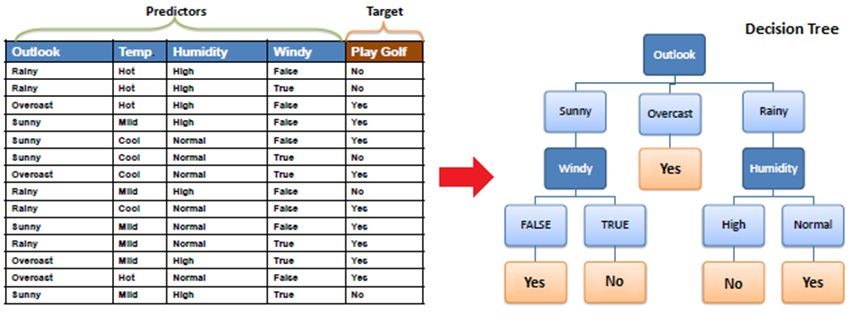
\includegraphics[width=0.8\textwidth]{recursos/arbol_decision_img1}
\label{fig:fun_arb_dec}
\end{figure*}
\FloatBarrier


\item Clasificación de Naïve Bayes.

Es un algoritmo que se basa en la técnica de clasificación utilizando el teorema de Bayes.

El algoritmo es capaz de agrupar un registro mediante las características de este. Para ello aplica probabilidades condicionales de las características para determinar a qué categoría pertenece. 

Por ejemplo, una fruta puede considerarse una manzana si es de color rojo, redonda y tiene un determinado peso.

\begin{figure*}[htb]
\centering
\caption{Teorema de Bayes. Recuperado de \protect\cite{uCincinnati2018}}
 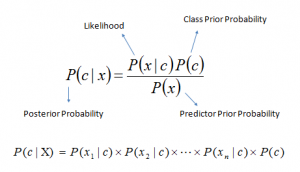
\includegraphics[width=0.6\textwidth]{recursos/BayesFormula}
\label{fig:BayesFormula}
\end{figure*}
\FloatBarrier

\item Regresión Logística

Es un algoritmo de regresión que se utiliza para predecir el resultado de una variable categórica en función de las variables independientes o predictores. Para predecir el resultado, se establecen pesos en función de la puntuación dada a cada variable independiente.

\item Redes Neuronales
%https://www.tuinteligenciaartificial.es/las-redes-neuronales-en-la-inteligencia-artificial-explicacion-clara-y-sencilla/

Las redes neuronales son un algoritmo de inteligencia artificial que se inspira en los mecanismos presentes en la naturaleza. Las neuronas envían señales eléctricas de manera fuerte o débil a otras neuronas. La combinación de todas las conexiones entre neuronas es lo que genera el conocimiento. Estas señales se envían cuando existe unos estímulos (inputs) externos a través de los sentidos. A lo largo de la vida, las neuronas aprenden que deben hacer a partir de dichos estímulos y, por lo tanto, los seres vivos aprenden a actuar ante distintas señales y situaciones. El funcionamiento de las redes neuronales en la inteligencia artificial es similar.

\begin{figure*}[htb]
\centering
\caption{Red Neuronal. Recuperado de \protect\citeA{yepes2017}}
 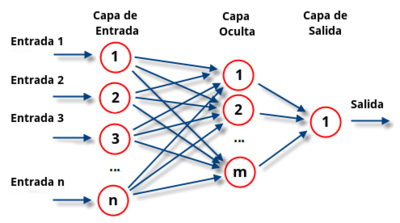
\includegraphics[width=0.6\textwidth]{recursos/RedNeuronalArtificial}
\label {fig:RedNeuronal}
\end{figure*}
\FloatBarrier

Como se puede observar en la figura \ref{fig:RedNeuronal}, la primera fila (con neuronas de color rojo), se conocen como nodos de entrada y son aquellos que se encargan de recoger la información. Los nodos en la gama azul son los que se conocen como nodos de salida. Los nodos situados en el medio son aquellos que se encargan de hacer el aprendizaje, y se conocen como nodos ocultos.

En primer lugar, se obtiene la información a partir de los nodos de entrada, una vez que se tiene la información, se envía a las capas ocultas, que se activan o no dependiendo del aprendizaje previo. Los nodos ocultos se activan dependiendo de una serie del resultado de unas operaciones matemáticas. Si los nodos se activan, entonces enviaran la información a la siguiente capa.

\item Bosques aleatorios

Los bosques aleatorios son un método que se encarga de combinar los resultados de árboles de decisión independientes.

Algunas características son:
\begin{itemize}
	\item Gran precisión.
	\item Eficiente para grandes bases de datos.
	\item Aporta estimaciones sobre la importancia de las variables en la clasificación.
	\item Tiene un método eficaz para la estimación de los datos faltantes y mantiene la precisión cuando falta una gran parte de los datos.
\end{itemize}
%https://quantdare.com/random-forest-vs-simple-tree/
%http://randomforest2013.blogspot.com/2013/05/randomforest-definicion-random-forests.html
%https://bookdown.org/content/2031/ensambladores-random-forest-parte-i.html

\item K-Vecinos-cercanos

K-vecinos-cercanos (conocido también como K-NN) es un algoritmo de aprendizaje supervisado en el que, a partir de unos datos iniciales, es capaz de clasificar todas las nuevas instancias.

La idea es que el algoritmo clasifica cada dato nuevo en el grupo que corresponda, según cual sea el grupo vecino (de los k grupos) mas próximo. Por tanto, calcula la distancia del elemento nuevo a cada uno de los existentes e indica a que grupo debe permanecer este nuevo elemento según la menor distancia.

\begin{figure*}[htb]
	\centering
	\caption{KNN. Recuperado de \protect\citeA{klein2018}}
	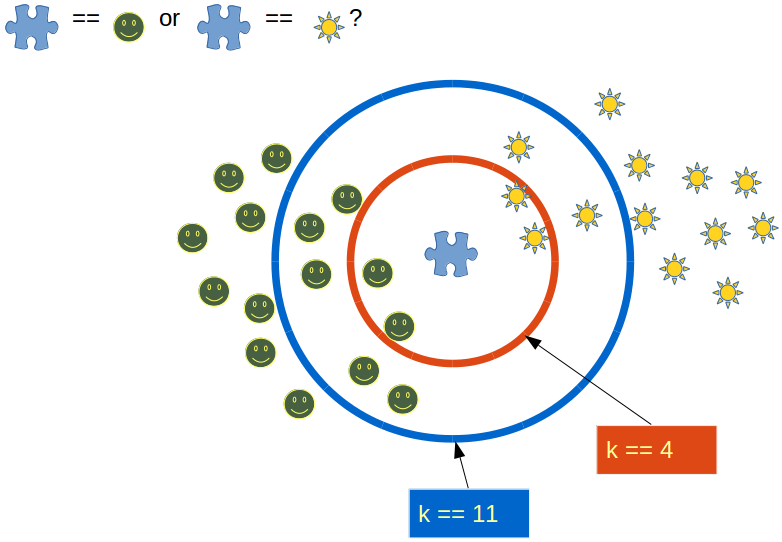
\includegraphics[width=0.6\textwidth]{recursos/k_NN}
	\label {fig:KNN}
\end{figure*}
\FloatBarrier


\end{enumerate}

\subsection{Distribución y Almacenamiento}
Respecto a la distribución de la información, esta no podrá salir de la consejería de educación. Aunque se trate de datos anonimizados y agregados, se trata de datos de carácter sensible y no pueden ser distribuidos. Por tanto, dichos datos se van a almacenar en un gestor de bases de datos MySQL. Este gestor se encontrará en un servidor de la Consejería de Educación. Solo se va a poder acceder a dicho servidor desde la propia sede. Es posible que los datos también se almacenen en archivos de texto plano.
